\documentclass[12pt,a4paper,titlepage]{article}
\title{Confronto fra algoritmo LMS e Fast Deconvolution per la cancellazione del crosstalk} 
\author{Matteo Orlandini}
\date{\today}

\usepackage[english, italian]{babel} %the last declared language is the one used in the document
\usepackage[utf8]{inputenc}
\usepackage[T1]{fontenc}
\usepackage{booktabs} %toprule, midrule, bottomrule
\usepackage{subfig}
\usepackage{graphicx}
\usepackage{listings}
\usepackage{siunitx}
\usepackage{amsmath}
\usepackage{mcode} % matlab code
%inizio impostazioni bibliografia
\usepackage[autostyle,italian=guillemets]{csquotes} 
%autostyle adatta lo stile delle citazioni alla lingua corrente del documento;
%italian=guillemets racchiude automaticamente tra virgolette caporali
%i campi che prevedono le virgolette;
\usepackage[backend=biber, style=numeric, citestyle=numeric,maxcitenames=99,maxbibnames = 99]{biblatex}
%backend=biber dice a biblatex che s’intende usare Biber come motore bibliografico
%style:numeric Anno di pubblicazione: in fondo al riferimento.
%citestyle=numeric Riferimento: numerico ([1], [2], eccetera).
%fine impostazioni bibliografia

\usepackage{float}
\usepackage{hyperref}
\hypersetup{
	bookmarks=true,         % show bookmarks bar?
	unicode=false,          % non-Latin characters in Acrobat’s bookmarks
	pdftoolbar=true,        % show Acrobat’s toolbar?
	pdfmenubar=true,        % show Acrobat’s menu?
	pdffitwindow=false,     % window fit to page when opened
	pdfstartview={FitH},    % fits the width of the page to the window
	%pdftitle={Relazione di Reti di Sensori Wireless per IOT},    % title
	pdfauthor={Matteo Orlandini},     % author
	pdfsubject= {Confronto fra algoritmo LMS e Fast Deconvolution per la cancellazione del crosstalk},   % subject of the document
	pdfcreator={Matteo Orlandini},   % creator of the document
	%pdfproducer={Producer}, % producer of the document
	pdfpagemode={UseOutlines},
	%bookmarksopen,
	pdfstartview={FitH},
	colorlinks=false,       % false: boxed links; true: colored links
	linkcolor={red},
	citecolor={green},
	urlcolor={cyan}
} 

\renewcommand{\lstlistingname}{Codice}

\addbibresource{Bibliografia.bib}

\newcommand{\CoverName}{Cover}

\begin{document}

\begin{titlepage}
	
	\centering
	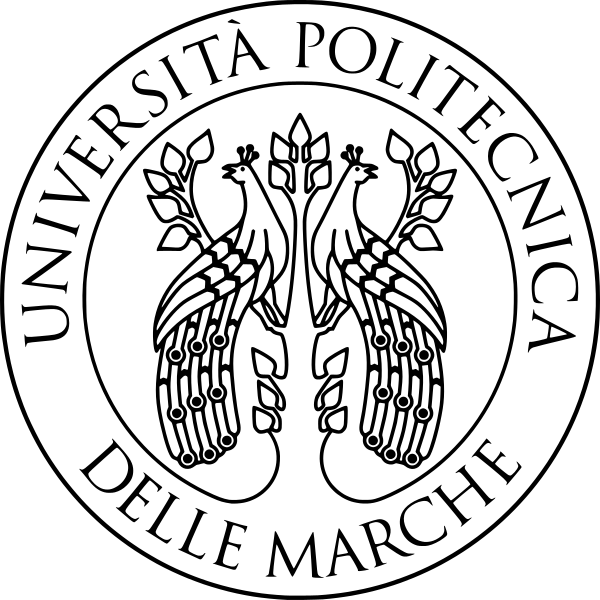
\includegraphics[width=.2\textwidth]{Immagini/univpmlogo}\par\vspace{1cm}
	{\scshape\LARGE Università Politecnica delle Marche\par}
	\vspace{1cm}
	{\scshape\Large Multirate Digital Signal Processing And Adaptive Filter Banks \par}
	\vspace{1.5cm}
	{\huge\bfseries Confronto fra algoritmo LMS e Fast Deconvolution per la cancellazione del crosstalk \par}
	\vspace{2cm}
	{\Large\itshape Matteo Orlandini e Jacopo Pagliuca\par}
	\vfill
	Prof.ssa Stefania \textsc{Cecchi}\\
	Dott.ssa Valeria \textsc{Bruschi}
	
	\vfill
	
	% Bottom of the page
	{\large \today\par}
\end{titlepage}

\thispagestyle{empty}
\tableofcontents

\newpage
\setcounter{page}{1}
\section{Introduzione}
\label{section:Introduzione}

\section{Dataset}
\label{section:Dataset}
Il dataset usato è composto ad un ampio set di \href{http://sound.media.mit.edu/resources/KEMAR/full.zip}{misurazioni della funzione di trasferimento relativa alla testa} (HRTF) di un microfono dummy-head KEMAR. Le misurazioni consistono nelle risposte impulsive dell'orecchio sinistro e destro di un altoparlante Realistic Optimus Pro 7 montato a 1,4 metri dal KEMAR. Sono state utilizzate sequenze binarie pseudo-casuali per ottenere le risposte impulsive a una frequenza di campionamento di \SI{44.1}{\kilo \hertz}. \cite{Gardner:HRTF}

Le misurazioni sono state effettuate nella camera anecoica del MIT. Il KEMAR è stato montato in posizione verticale su un giradischi motorizzato che può essere ruotato con precisione sotto il controllo del computer. L'altoparlante è stato montato su un supporto a braccio che ha consentito il posizionamento accurato dell'altoparlante a qualsiasi elevazione rispetto al KEMAR. Pertanto, le misurazioni sono state effettuate un'elevazione alla volta, impostando l'altoparlante all'altezza corretta e quindi ruotando il KEMAR su ciascun azimut.

I dati HRTF vengono archiviati nelle directory per elevazione. Ogni nome di directory ha il formato "elevEE", dove EE è l'angolo di elevazione. All'interno di ogni directory, il nome di ogni file ha il formato "XEEeAAAa.wav" dove X può essere "L" o "R" rispettivamente per la risposta dell'orecchio sinistro e destro, "EE" è l'angolo di elevazione della sorgente in gradi, da -40° a 90°, e AAA è l'azimut della sorgente in gradi, da 0° a 355°. Gli angoli di elevazione e azimut indicano la posizione della sorgente rispetto al KEMAR, in modo che, ad esempio, in corrispondenza dell'elevazione 0 e azimut 0 sia di fronte al KEMAR , l'elevazione 90 è direttamente sopra il KEMAR, elevazione 0 e azimut 90 è a destra del KEMAR. Ad esempio, il file "R-20e270a.wav" è la risposta dell'orecchio destro, con la sorgente 20 gradi sotto il piano orizzontale e 90 gradi a sinistra della testa.

\clearpage

\nocite{*}
%Il comando \printbibliography produce la sezione bibliografica con relativi
%titolo e testatina. Per mandarne il relativo titolo nell’indice generale si
%usa l’istruzione:
\printbibliography

\end{document} 